\documentclass[12pt, a4paper, notitlepage, oneside]{article}
\usepackage[english]{babel}
\usepackage[utf8]{inputenc} 
\usepackage{graphicx}
\usepackage{hyperref}
\usepackage{enumerate}
\usepackage{setspace}
%\singlespacing

\makeatletter

\newcommand{\linia}{\rule{\linewidth}{0.4mm}}

\renewcommand{\maketitle}{
\begin{titlepage}

    \vspace*{1cm}

    \begin{center}\small

    Warsaw University of Technology\\
    The Faculty of Electronics and Information Technology\\

    \end{center}

    \vspace{3cm}

     \begin{center}

    Data Mining (EDAMI)\\ Project Documentation

    \end{center}

    \noindent\linia

    \begin{center}

      \LARGE \textsc{\@title}

         \end{center}

     \noindent\linia

    \vspace{0.5cm}

    \begin{flushright}

    \begin{minipage}{5cm}

    \textit{\small Authors:}\\

    \normalsize \textsc{\@author} \par

    \end{minipage}

    \vspace{4cm}
    
 

     \end{flushright}

    \vspace*{\stretch{6}}

    \begin{center}

    \@date

    \end{center}

  \end{titlepage}
}

\makeatother

\title{Clustering based on density}

\author{Aleksandra Kurdo\\ Adam Stelmaszczyk}

\begin{document}

\maketitle


\onehalfspacing


\section*{Project task}
Implementation and experimental evaluation of DBSCAN~\cite{dbscan} and DENCLUE~\cite{denclue} algorithms. 

\section*{Solution specification}

\subsection*{Data set}~\cite{dataset}

Set with information about geometrical properties of kernels belonging to three different varieties of wheat was chosen.

\subsubsection*{Data set attribute information}


To construct the data, seven geometric parameters of wheat kernels were measured: 

\begin{itemize}
	\item area A, 
	\item perimeter P, 
	\item compactness C, 
	\item length of kernel, 
	\item width of kernel, 
	\item asymmetry coefficient 
	\item length of kernel groove. 
\end{itemize}

All of these parameters were real-valued continuous.


\subsection*{Algorithms description}
 
\subsubsection*{DBSCAN algorithm}





\subsubsection*{DENCLUE algorithm}

Denclue algorithm is based on the idea that the influence of each data point can be modeled using a mathematical function (influence function). The overall density of the data space can be calculated as the sum of the influence function of all data points. Clusters can be determined mathematically by identifying density-attractors, which are the local maxima of the overall density function.

The Denclue algorithm works in two steps. 

Step one: 

\begin{itemize}
	\item It is preclustering step, in which a map of the relevant portion of the data space is constructed. The map is used to speed up the calculation of the density function which requires to efficiently access neighboring portions of the data space. 
\end{itemize}


Step two:

\begin{itemize}
	\item It is the actual clustering step, in which the algorithm identifies the density-attractors and the corresponding density-attracted points.
\end{itemize}

\subsection*{Implementation details}

As implementation language for the project Java was chosen. Data set is read from a text file, that located in program root folder, and a set of objects that represent points is generated. On this set Dbscan and Denclue algorithms are runs. Other arguments that algorithms need are declared directly in the program files.

Program consists from five packages:
\begin{itemize}
	\item algorithms package. In this package abstract class ClusteringAlgorithm and inherited from it classes Dbscan and Denclue are located. 

	\begin{figure}[!ht]
 	\centering
	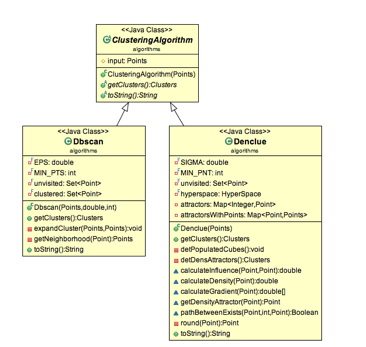
\includegraphics[width=0.8\textwidth]{images/algorithms_package.png}
 	\caption[]
	{Class diagram for algorithms package}
	\end{figure}


	\item structures package. Here are located classes Cluster, Point and Points, that used simply to describe set of points and generated clusters. 

	\begin{figure}[!ht]
 	\centering
	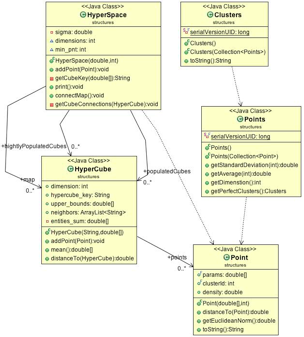
\includegraphics[width=0.8\textwidth]{images/structures_package.png}
 	\caption[]
	{Class diagram for structures package}
	\end{figure}

	\item scorer package. This package consists of a class Scorer, that used to generate some statistics about created by algorithm clusters.

	\begin{figure}[!ht]
 	\centering
	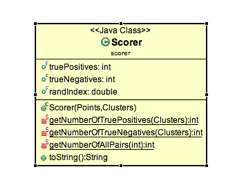
\includegraphics[width=0.6\textwidth]{images/scorer_package.png}
 	\caption[]
	{Class diagram for scorer package}
	\end{figure}

\item visualizer package. Used for  the clusters visualization.

	\begin{figure}[!ht]
 	\centering
	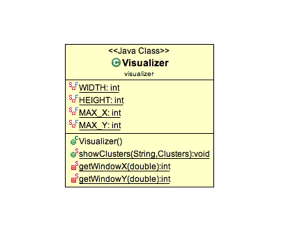
\includegraphics[width=0.6\textwidth]{images/visualizer_package.png}
 	\caption[]
	{Class diagram for visualizer package}
	\end{figure}

\item main package. Used for  reading the data set from the file and executing algorithms.

	\begin{figure}[!ht]
 	\centering
	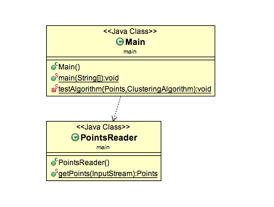
\includegraphics[width=0.8\textwidth]{images/main_package.png}
 	\caption[]
	{Class diagram for main package}
	\end{figure}


\end{itemize}


\subsection*{User guide}

\subsection*{Experimentation results and analysis}

As a result of execution Dbscan and Denclue algorythms two sets of clusters are generated. This clusters are represented as points in 2D view as a set of points that belong to them. Each point represented as a number of it’s cluster. Data set attributes area and asymmetry coefficient are chosen as a dimensions of the view.

\begin{figure}[!ht]
 	\centering
	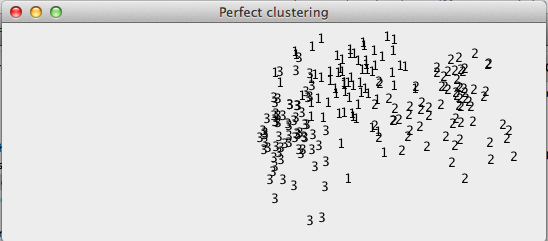
\includegraphics[width=0.8\textwidth]{images/perfect.png}
 	\caption[]
	{Class diagram for main package}
	\end{figure}

\begin{figure}[!ht]
 	\centering
	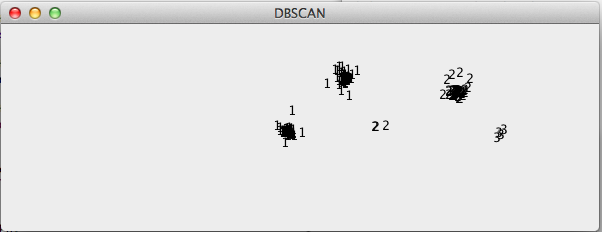
\includegraphics[width=0.8\textwidth]{images/dbscan.png}
 	\caption[]
	{Class diagram for main package}
	\end{figure}

\begin{figure}[!ht]
 	\centering
	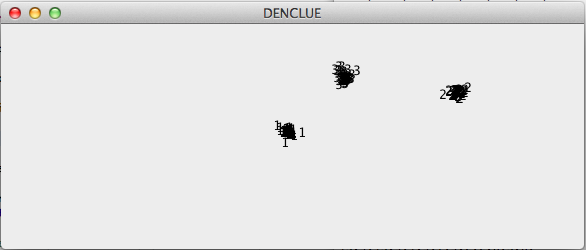
\includegraphics[width=0.8\textwidth]{images/denclue.png}
 	\caption[]
	{Class diagram for main package}
	\end{figure}


%\begin{figure}[!ht]
 % \centering
%  \includegraphics[width=1\textwidth]{images/ex_locations.png}
 % \caption[]
%  {Example}
%\label{ex_}
%\end{figure}


%\url{http://archive.ics.uci.edu/ml/machine-learning-databases/00236/} 

\bibliographystyle{plain}
\bibliography{references}
\end{document}